\chapter{Implementation}
This chapter is dedicated to presenting a prototype implementation of the
previously discussed designs within the gem5 simulator. The main goal here is to
provide a comprehensive overview of critical implementation details, showcasing
how these designs are brought to life within the gem5 environment. It will also
highlight the addition of new instructions to the compiler, which are used by
the software that runs on the gem5 simulator. 

\section{Mode Switch Mode}

\begin{figure}[h]
    \centering
    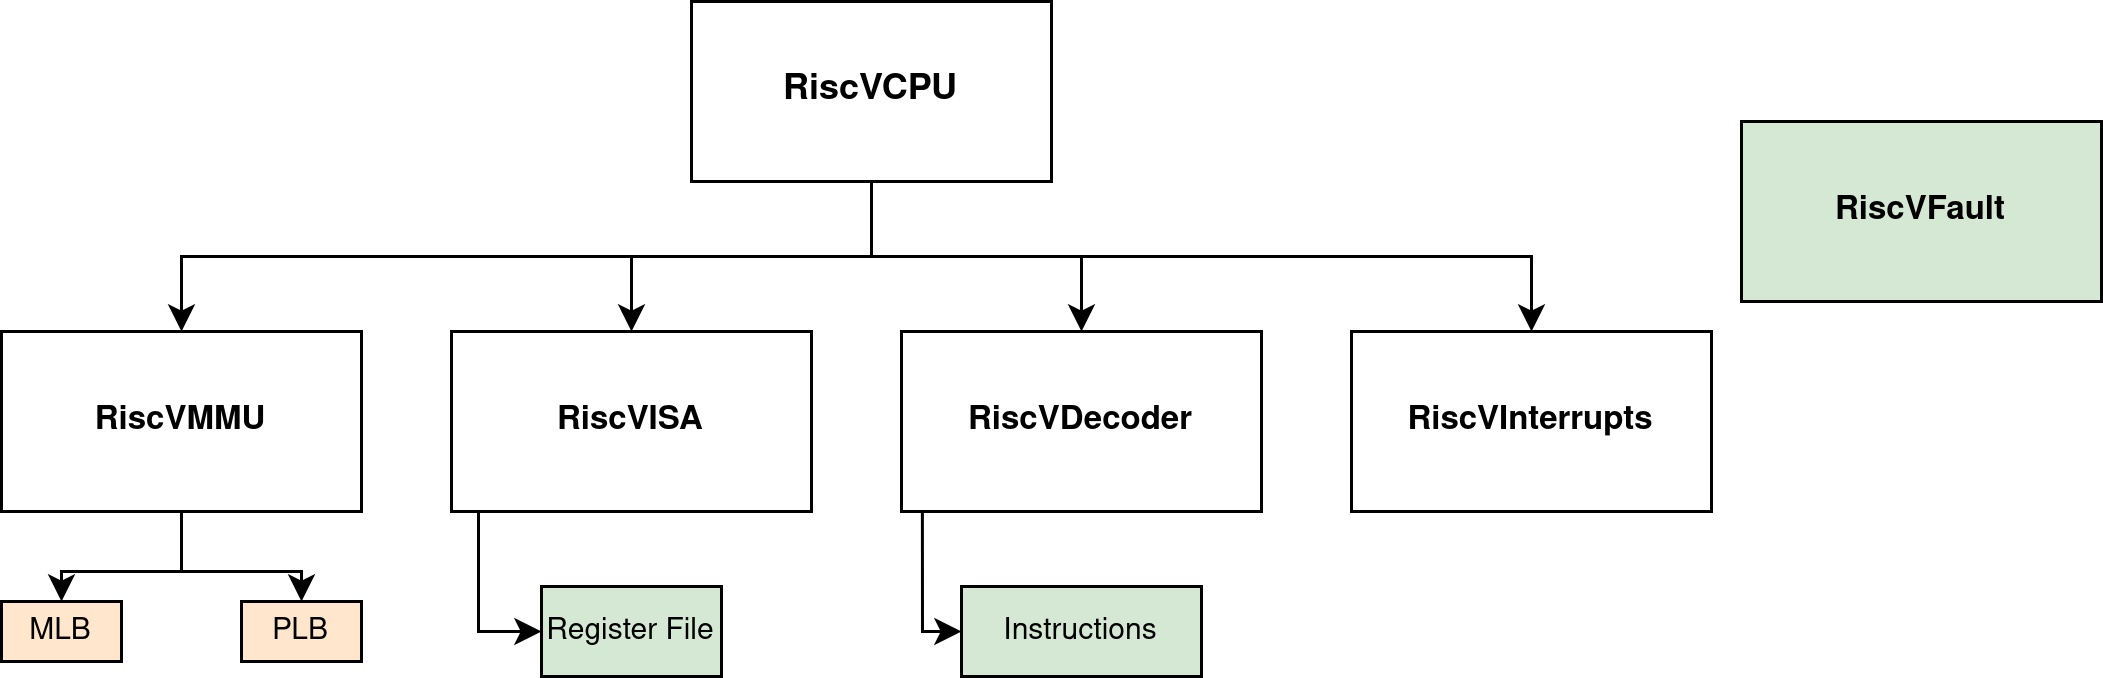
\includegraphics[width=1\textwidth]{overview_im}
    \captionsetup{justification=centering}
    \caption{Overview over the gem5 Risc-V building blocks}
            Yellow symbolizes elements that are newly added, green marks
            elements which were in the original Risc-V implementation and have
            now a slightly different one. 
    \label{fig:overview_im}
\end{figure}

The gem5 simulator has already implemented Risc-V as a usable processor type.
This processors internal structure comprises multiple interconnected C++ classes
and is utilized within simulations as a Python Class. When employing
this processor in a simulation, it instantiates a Risc-V CPU, serving as the
primary implementation of the Risc-V architecture within gem5. This CPU
comprises four primary modules: the Risc-V MMU, Risc-V ISA, Risc-V Decoder, and
Risc-V Interrupts (refer to Fig.\ref{fig:overview_im}). The RISC-V MMU managed
memory requests and acting as an interface between CPU, memory and caches.
The Risc-V ISA module manages the CPU's state, including control over the
program counter, outstanding faults, and crucially, the CPU registers. It
provides an interface to interact with these registers, considering the
potential side effects of such interactions, including checks against privilege
levels. Consequently, any register implementation occurs within this module. The
Risc-V Decoder interprets the incoming binary instruction stream, employing
auto-generated execution modules to execute individual instructions. The
instructions are defined in a specialized ISA description language,
which is the most important aspect of implementing new instructions.
Another crucial component is the Risc-V Fault module, encompassing events triggered by
the simulation to manage the changes that any kind of fault induces
within the CPU. This module is essential for facilitating transitions into the
Mode Switch Mode. The Risc-V Interrupts module primarily checks for interrupt occurrences and
triggers a fault event if such a check confirms an interrupt. Additionally, it
sets a bitmask within certain control and status registers. While minor
adjustments are made to the bitmask, the majority of this module remains
unchanged for this specific work.\par
I adopted the solution proposed by Von Elm et al.\cite{Cve} for both MLB and PLB,
seamlessly integrating it into the MMU of the RISC-V CPU. This implementation
was employed to access Memory Lookaside Buffers (MLB) and Permission Lookaside
Buffers (PLB) while handling instructions. In each pagetable walk conducted by
the pagetable walker integrated into the MMU, the PLB is utilized to verify
segmentation rights. The inclusion of the MLB in the MMU is justified by its
role as a cache for modes, making it appropriate for implementation within the
module responsible for managing these aspects. To align with the specifications
outlined in the design chapter, I introduced minor modifications to the entries
for encoding relevant information. Additionally, within the MLB, I introduced a
method \texttt{can\char`_access\char`_csr} which takes a mode ID and a CSR number as inputs,
verifying whether the mode possesses the necessary access rights to the CSR.
This method emulates a hardware check performed by the MLB.\par
Within the Risc-V ISA module, I removed all references and checks related to
modes. I augmented the \texttt{vector} that defines the CSRs
by introducing new fields representing the \texttt{prv} and
\texttt{mode} registers. Upon initialization, the current mode is set to the
Mode Switch Mode instead of machine mode.\par
In the Risc-V Decoder, specifically in the ISA description, I modified all existing
functions that read or write a CSR to validate if such operations are
allowed in the current mode. This validation is achieved by calling
\texttt{can\char`_access\char`_csr} from the MLB with the current mode and the
CSR intended for access. Furthermore, I included the new instructions introduced
in the design chapter.\par
Significant modifications were made in the Risc-V Fault module. All alterations
specific to modes in certain registers or the CPU state were removed. Instead
the Mode Switch Mode is entered without any changes to the current registers. To
do this the program counter, which is reset here, is set to the entry point of
the Mode Switch Mode. The mode which is left is saved to the \texttt{mode} field
in the CSR vector while the \texttt{prv} field is set to 1 which represents the
Mode Switch Mode. These module changes apply solely to the full system
simulation, as only this simulation replicates CPU changes.\par 

\section{Control Core}
For the Control CPU, I opted to employ two Risc-V processors, both implementing
the Mode Switch Mode. Certain alterations were made to the ISA, which I will
elaborate on later. Firstly, I aim to clarify the overall structure necessary to
realize this design.\par 
As depicted in Figure \ref{fig:python_im}, I interconnected two Risc-V CPUs
through a crossbar, establishing a link to the main memory. Alongside these two
CPUs, there exists two PIO devices connected to the same crossbar. One of the CPUs is
designated as the main CPU, while the other serves as the Control Core. The PIO
devices, which respond to writes at specific addresses, function as handlers for
both CPUs. In the event of a trap occurring at the main CPU, the RiscVFault
module is configured to issue a write to the \emph{main CPU} PIO device's address, activating
it. Subsequently, this PIO device deactivates the main CPU and sets the program
counter of the Control Core to a fixed handler address. The Control Core's
wake-up is scheduled using a gem5 event. Activating the Control Core through a
gem5 event offers the advantage of introducing a customizable delay. The return
path from the Control Core to the main CPU follows a similar procedure. Once the
Control Core completes its execution, it returns to the main CPU using the \texttt{mret}
instruction. This instruction triggers a write to the \emph{cc} PIO device's address
causing the PIO device to deactivate the Control Core and activate
the main CPU through another gem5 event. The main CPU then resumes execution in
its current state, configured appropriately by the code on the Control Core.
The decision to implement two fully developed CPUs was driven by the ability to
write code for the Control Core in standard RiscV assembly and leverage the
existing toolchain for building on it. This system configuration was established
using the gem5 python build tools.\par

\begin{figure}[h]
    \centering
    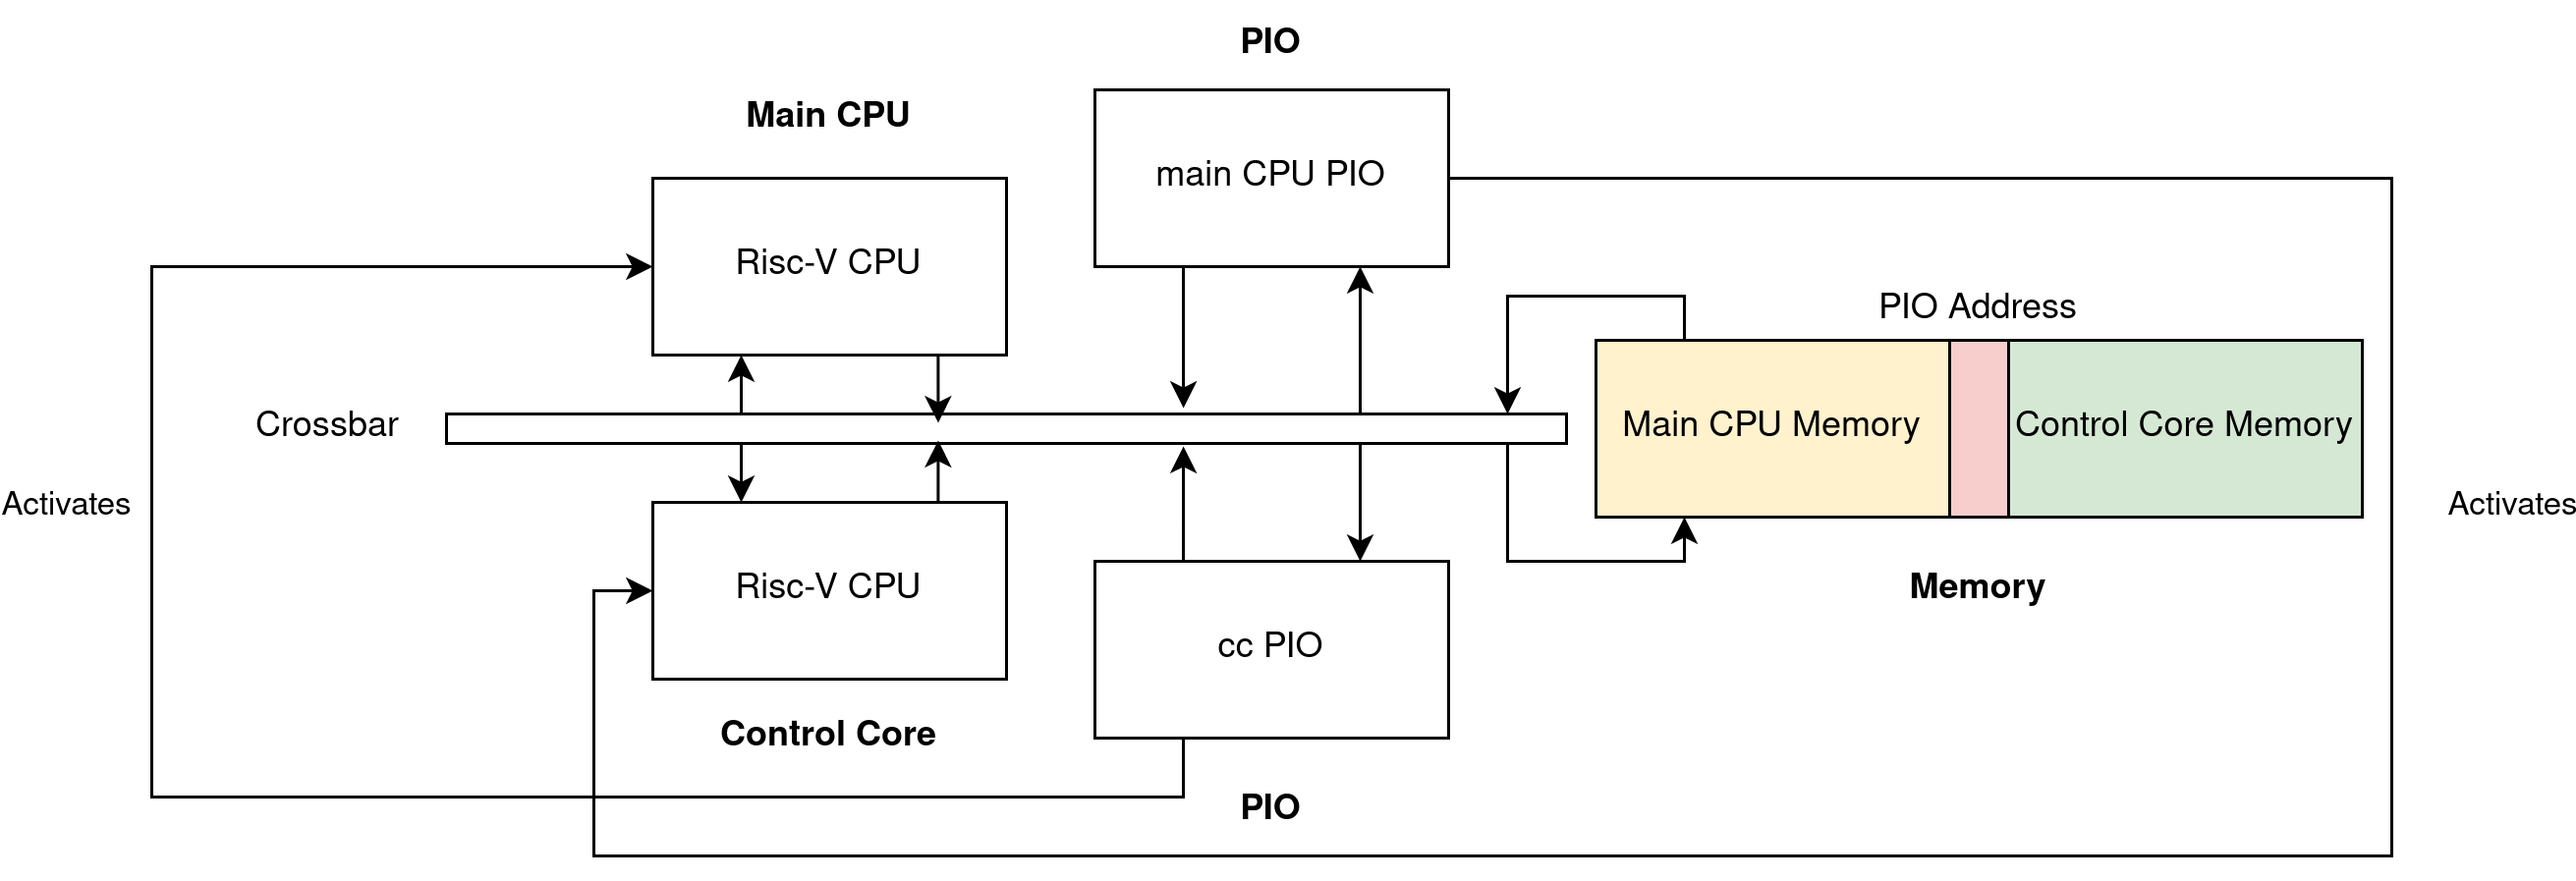
\includegraphics[width=1\textwidth]{python_im}
    \captionsetup{justification=centering}
    \caption{Schema of the Control Core}
        Two dedicated memories for each subsystem for memory isolation. The PIO
        device activates the CPUs of the different systems.
    \label{fig:python_im}
\end{figure}

Within the Risc-V ISA module, a new pointer named \texttt{foreign\char`_isa} is introduced.
This pointer stores a reference to the Risc-V ISA module of another CPU. During
simulation setup, this pointer is initialized with a reference to the Risc-V ISA
module of the other of the two CPUs. This allows access to the registers of the other CPU
through special instructions described in the design chapter. These instructions are
implemented within the ISA description of the Risc-V Decoder. Ordinarily, a
register-altering instruction invokes one of the register access functions of
the current ISA. However, an instruction accessing the registers of the other
CPU uses the \texttt{foreign\char`_isa} to invoke the same functions on the other
CPU. Instructions utilizing this pointer are limited to the Control Core, and if
employed on the main CPU, they result in an illegal instruction fault.

\section{Compiler Instructions}
To facilitate the utilization of the newly introduced instructions, I opted to
integrate them into the GNU assembler. This integration requires four key
components: the instruction's name, format, mask, and match. The RISC-V project
provides the riscv-opcodes tool, enabling the derivation of the mask and match
for an instruction from its string representation. Once obtained, along with the
instruction's name and format, these components can be seamlessly implemented
directly into the GNU assembler. This integration enhances the ease of use for
developers leveraging the modified instruction set within the GNU assembler
environment.